\chapter{Avaliação}

Neste capítulo, será mostrado os resultados da aplicação do software em um contexto real, ou seja, o software foi
utilizado na disciplina de Teste de Software do curso de engenharia de software na universidade de brasília campus
de engenharias gama. O capítulo está dividido em seções que estão disposta da seguinte maneira: na seção 5.1 será mostrado
uma pequena introdução sobre os questionários de avaliação, na seção 5.2 será será listado os cenários de avaliação, na
seção 5.3 será mostrado o questionário de avaliação e na seção 5.4 o resultado da avaliação.

\section{Questionários de Usabilidade}

Uma parte importante da engenharia de produtos é a medida de usabilidade. Os métodos de medição para avaliar a
usabilidade não são óbvios e são um preocupação permanente dos engenheiros. A maioria das avaliações de usabilidade
reúne dados quantitativos subjetivos e objetos no contexto de cenários realistas de uso. Os dados subjetivos são medidas
das opniões ou atitudes dos participantes em relação a sua percepção de usabilidade, já os objetivos são medidas do
desempenho dos participantes como tempo de conclusão, taxa de sucesso e etc \cite{questionario}.

Como o objetivo do software é automatizar e aumentar a satisfação do uso de metodologias ativas de aprendizado as
medidas subjetivas terão maior consideração na avaliação do mesmo. As medidas subjetivas são geralmente respostas a
itens do questionário do tipo "\textit{like}" que avaliam atitudes do usuário em relação a atributos como facilidade de uso do
sistema e a similaridade de interfaces em determinados cenários. A maioria dos cenários de avaliação de usabilidade são
conjuntos de tarefas nas quais os usuários resolvem problemas, por exemplo, como resolver a lista de exercício, se
preparando para as avaliações, automatizar o cálculo das notas entre outras em relação aos requisitos não funcionais \cite{questionario}.

Para adquirir essas métricas será utilizado um questionário da IBM especificamente para uso no contexto de testes de
usabilidade baseados em cenários e medidas subjetivas. Foi analisado alguns tipos de questionários como o
\textit{After-Scenario Questionnaire} (ASQ), \textit{Printer Scenario Questionnaire} (PSQ), \textit{Post-Study System
Usability Questionnaire} (PSSUQ) e \textit{Computer System Usability Questionnaire} (CSUQ). Como as metodologias ativas
de aprendizado tem alguns cenários que precisam ser avaliados separadamente, foi definido para a avaliação de satisfação
dos usuários o questionário ASQ, pois ele é um questionário curto e consegue adquirir métricas para cada cenário do
software. Apesar de o ASQ e o PSQ terem os mesmo itens mudando apenas a escala de avaliação, o ASQ tem uma
confiabilidade melhor de acordo com \cite{questionario}. Já o PSSUQ e o CSUQ são ambos questionários gerais de
satisfação, ou seja, são questionários mais extensos que englobam todo o sistema, que não é o ideal para a avaliação, já
que não conseguiria coletar feedbacks de cada cenário para possíveis melhorias.

\section{Cenários de avaliação}

Abaixo será listado os cenários de avaliação na qual será aplicado o questionário ASQ em comparação ao mesmo cenário sem
utilizar o softwate PGTBL.

\begin{itemize}
  \item avaliação iRAT
  \item avaliação gRAT
  \item avaliação prática
  \item avaliação em pares
  \item cálculo das notas
\end{itemize}

Os 4 primeiros itens são questionários para o estudante responder depois de cada cenário, o quinto item é
para o professor responder após a conclusão do TBL.

\section{Questionário ASQ}

O questionário Pós-cenário (ASQ) é um questionário de três ou mais itens que os avaliadores de usabilidade da IBM utilizam para
avaliar a satisfação do participante após a conclusão de cada cenário proposto \cite{questionario}. Os itens do
questionário abordam afirmações relacionadas a 4 dos 5 requisitos não funcionais aplicados a ferramenta para avaliar se
os requisitos foram satisfeitos. Os requisitos são: suportabilidade, desempenho, usabilidade e segurança ou
confiabilidade. O quinto requisito não funcional, o requisito de qualidade, é respondido pelas métricas
coletadas na ferramenta codacy.

O questionário será constituido de itens com escalas gráficas de 7 pontos, na qual temos 7 para o caso do usuário concordar
totalmente e 1 caso discordar totalmente e um ponto não aplicavel (N/A) fora da escala para o caso de o usuário não
querer responder. O resultado será a média aritmética dos escores dos quatro itens para obter a pontuação do ASQ para a
satisfação de um participante com o sistema para um determinado cenário. Quanto mais alto o resultado melhor. Se um
participante não responder a um item ou marcar N/A, o cálculo da média será a média dos itens respondidos.

$$P_{i} = \frac{x_{1} + x_{2} + x_{3} + x_{4}}{4}$$

$$R_{final} = \sum_{i=1}^{n} \frac{P_{i}}{n}$$

$P_i$ é a pontuação final de cada aluno no questionário, $x$ é a pontuação de cada item do questionário, $R_{final}$ é o resultado final da avaliação de usabilidade,
$i$ é o indice de cada aluno e $n$ é a quantidade total de alunos.

Questionário para cada cenário:

Em relação ao software PGTBL para cada uma das afirmações abaixo, preencha a classificação de sua escolha.

\begin{figure}[h!]
  \centering
  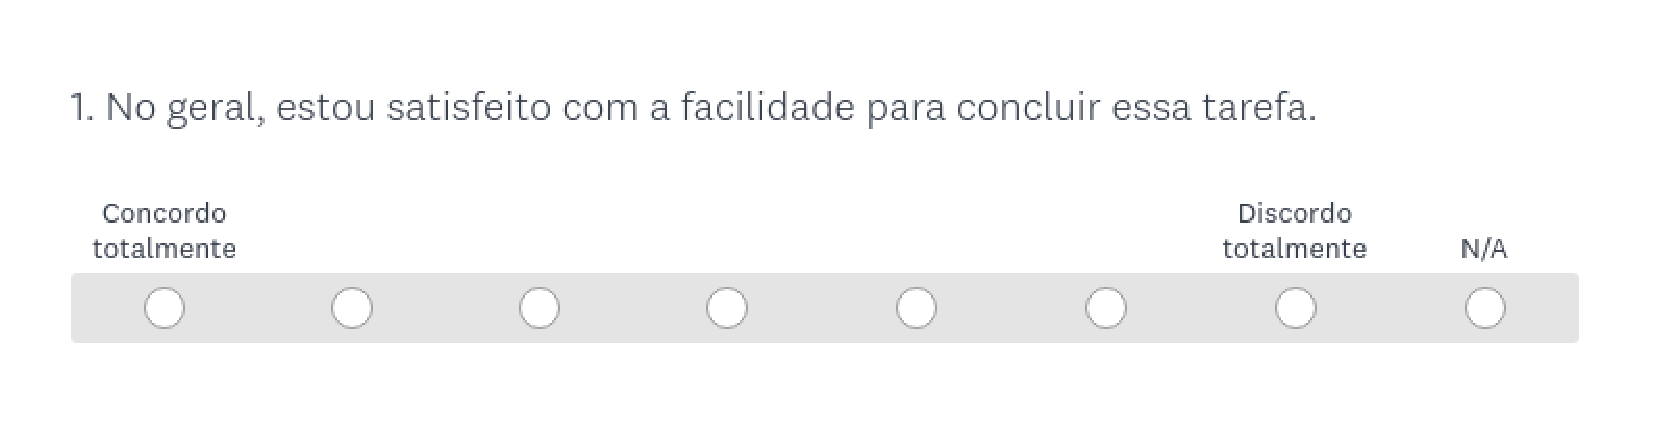
\includegraphics[keepaspectratio=true,scale=0.5]{figuras/p1.eps}
\end{figure}

\begin{figure}[h!]
  \centering
  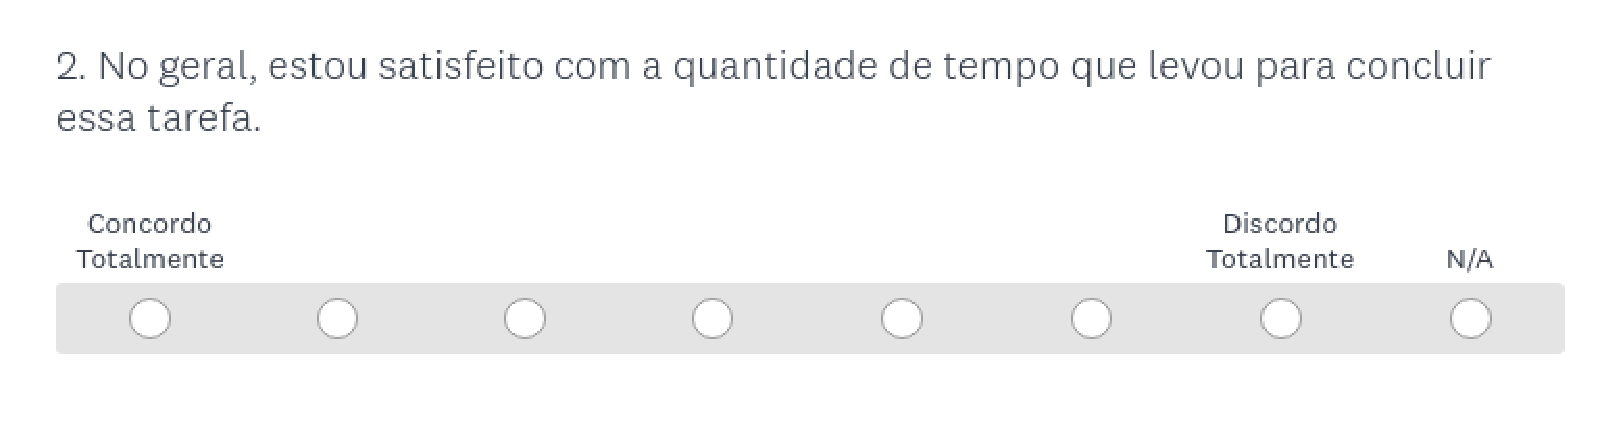
\includegraphics[keepaspectratio=true,scale=0.5]{figuras/p2.eps}
\end{figure}

\begin{figure}[h!]
  \centering
  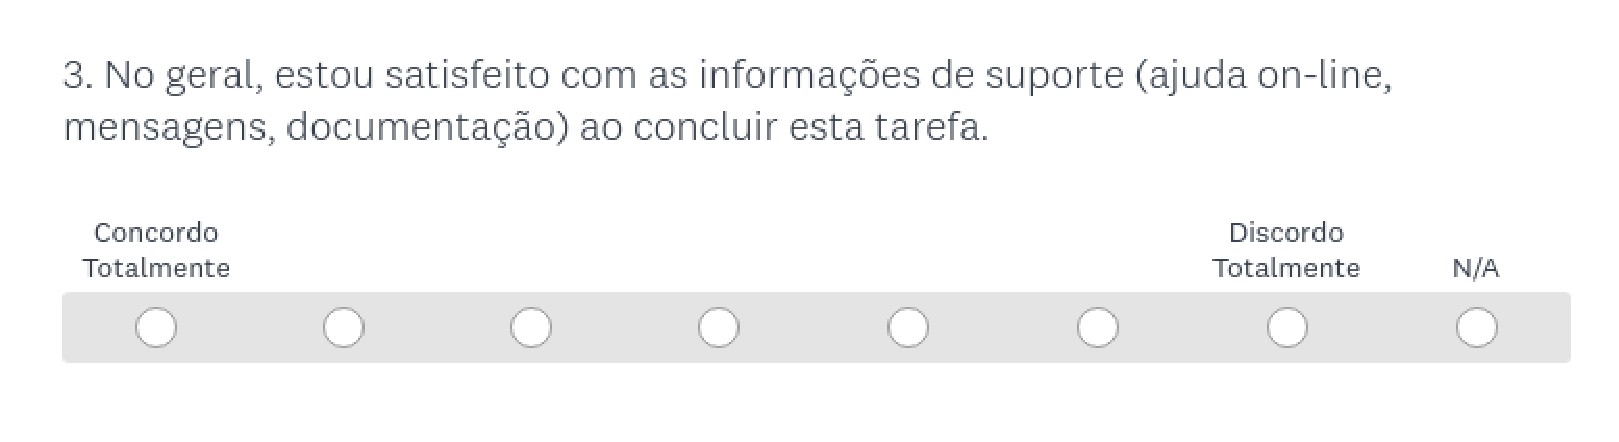
\includegraphics[keepaspectratio=true,scale=0.5]{figuras/p3.eps}
\end{figure}

\begin{figure}[h!]
  \centering
  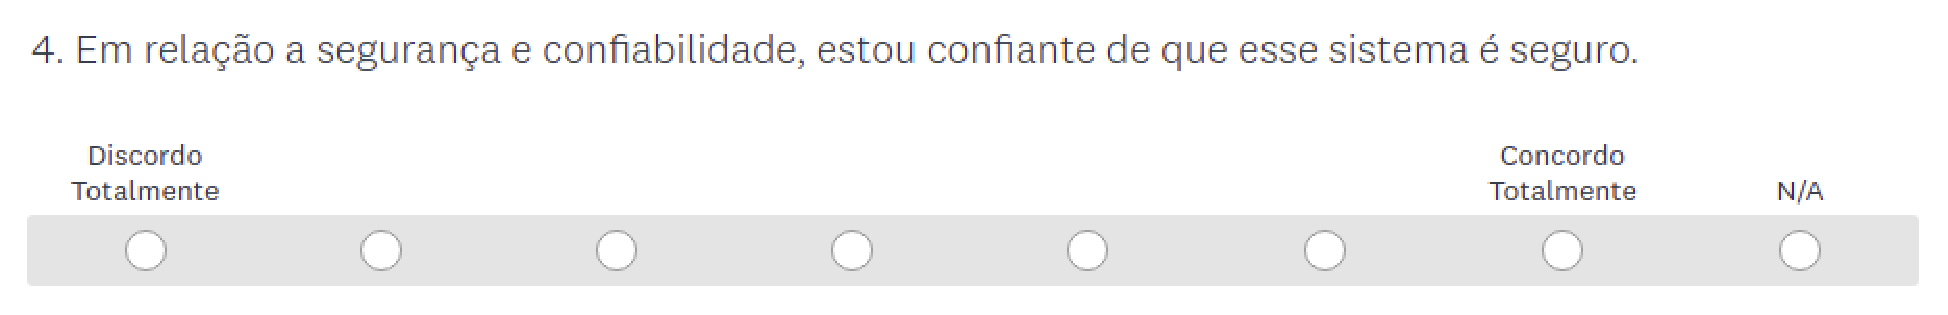
\includegraphics[keepaspectratio=true,scale=0.5]{figuras/p4.eps}
\end{figure}

\section{Resultado}

...
